\documentclass{article}

\usepackage{pythontex}
\setpythontexoutputdir{.} % This is the important bit, when building into separate build directory!

\usepackage{graphicx}
\graphicspath{{./}}

\newcommand{\pymultiply}[2]{\py{#1*#2}}

\begin{document}

\begin{pycode}
print("Python says Hello!")
\end{pycode}

\(8 \times 256 = \pymultiply{8}{256}\)

\begin{figure}
    \centering
    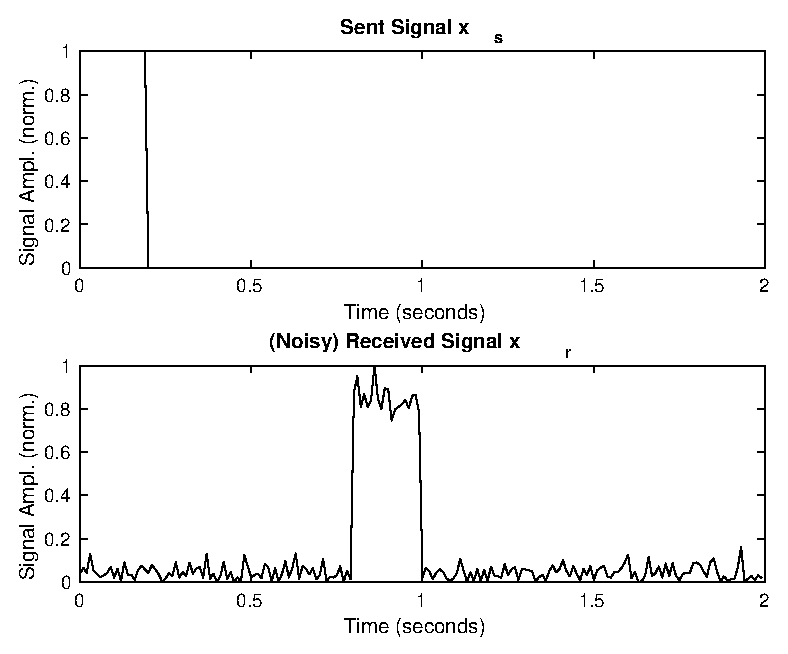
\includegraphics[width=\textwidth]{signals}
    \caption{This should be a graph of two signals.}
\end{figure}

\end{document}
